\documentclass[11pt]{article}
\usepackage{fullpage,url}
\usepackage{amsmath}
\usepackage{graphicx}  

\usepackage[letterpaper,top=1in,bottom=1in,left=1in,right=1in,nohead]{geometry}

\setlength{\parindent}{0in}
\setlength{\parskip}{6pt}

\DeclareMathOperator{\E}{E}
\DeclareMathOperator{\Var}{Var}
\DeclareMathOperator{\Unif}{Unif}

\begin{document}
\thispagestyle{empty}
{\large{\bf CSE 586A  \hfill Your Name Here!!}}\\

{\LARGE{\bf Problem Set I}}
\vspace{0.2\baselineskip}
\hrule

The purpose of this template is to get you started on the LaTeX for the problem sets. 
Feel free to use as much as you want, or start from scratch if you prefer. Obviously, you
need to delete all of the text I have giving advice throughout. Just make sure that your
write-up is formatted nicely and the solutions are clear. That is to say, you should explain everything
well enough concisely. Please do not write me a $20$ page document!

It's good to repeat and state briefly each problem before diving into the answer. For example:
\begin{enumerate}

\item
\begin{enumerate}
\item Here I prove that $\E[ \E[X | Y] ] = \E[X]$.\\

You might use the {\tt align} environment for this type of problem. For example:
\begin{align*}
\E[\E[X | Y]] &= \E \left[ \int_{-\infty}^\infty x \, p(x | y) \, dx \right] &
\text{definition of} \E[X | Y] \\
&= \text{next equation} & \text{explain this step}\\
&= \text{next equation} & \text{explain this step}\\
&= \E[X]
\end{align*}

Note: {\tt align*} environment will not number the lines, but {\tt align} will
add equation numbers. Also, when doing a derivation like this, you should
{\em always} explain what you are doing. You don't have to necessarily add an
explanation for every line (like above), that is, you don't have to explain
obvious or trivial steps. If you are unsure, add an explanation! Also, it
doesn't necessarily have to be inline with the equation, you can explain it in a
sentence or two, before/after the equation.

\item Here I prove that $\Var(X) = \E[\Var(X | Y)] + \Var(\E[X | Y])$.\\

We first expand the two terms on the right-hand side:
\begin{align*}
\E[\Var(X | Y)] &= \ldots & \text{explain}\\
&= \ldots & \text{explain}
\end{align*}

\begin{align*}
\Var( \E[X | Y] ) &= \ldots & \text{explain}\\
&= \ldots & \text{explain}
\end{align*}

Putting these together, we have
\begin{align*}
\E[\Var(X | Y)] + \Var( \E[X | Y] ) &= \text{plug in formulas above} & \text{explain}\\
&= \text{simplify...}  & \text{explain}\\
&= \Var(X)
\end{align*}

\end{enumerate}

%% Problem 2
\item Let $X \sim \mathrm{Exp}(\lambda)$, and let $Y = \sqrt{X}$.
\begin{enumerate}
\item %% (a)

\item %% (b)

\item %% (c)

\item %% (d)
\end{enumerate}

\item Start with defining $\ln L(\lambda ; y_1, \ldots, y_n)$, and then maximize
with respect to $\lambda$.

If want to include a figure, then use the following lines:
\begin{figure}[h!]
\begin{center}
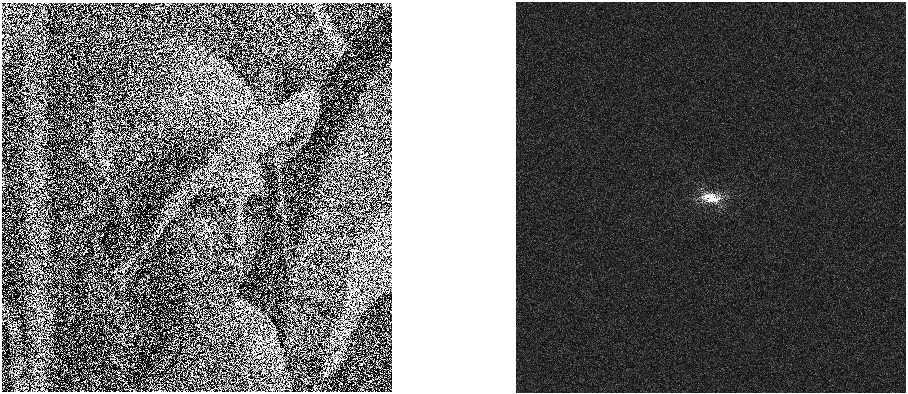
\includegraphics[width=0.6\textwidth]{fft_noise}
\caption{Always write a caption!!}
\label{fig:fouriertransform}
\end{center}
\end{figure}

Note that the figure format is {\tt .pdf}. You can also use other different image format, such as PNG or JPEG
for your graphics. You can reference a figure in the text like this: Figure~\ref{fig:fouriertransform}.

\end{enumerate}

\end{document}
